\documentclass[11pt,a4paper]{article}
\usepackage{fontspec}
\setmainfont{NotoSerifCJKkr-Regular.otf}[Path=fonts/,BoldFont=NotoSerifCJKkr-Bold.otf,ItalicFont=NotoSerifCJKkr-Regular.otf]
\setsansfont{NotoSerifCJKkr-Regular.otf}[Path=fonts/,BoldFont=NotoSerifCJKkr-Bold.otf]
\setmonofont{DejaVu Sans Mono}[Scale=0.79]
\XeTeXlinebreaklocale "ko"
\XeTeXlinebreakskip=0pt plus 1pt
\usepackage[margin=23mm,top=23mm,bottom=23mm,headheight=15pt]{geometry}
\usepackage{amsmath,amssymb,amsthm,mathtools}
\usepackage{booktabs,tabularx,longtable,array,graphicx,float}
\usepackage[dvipsnames]{xcolor}
\usepackage{enumitem,caption,fancyhdr,titlesec}
\usepackage{tikz}
\usetikzlibrary{arrows.meta,positioning,calc}
\usepackage{hyperref}
\hypersetup{unicode=true,colorlinks=true,linkcolor=MidnightBlue,urlcolor=MidnightBlue,citecolor=MidnightBlue,pdftitle={WU088 HH PHYS16: 상관된 endpoint 결함과 유한 adjoint 나머지},pdfauthor={WU088 HH 연구}}
\urlstyle{same}
\setlength{\emergencystretch}{3em}
\setlength{\parskip}{0.34em}
\setlength{\parindent}{1em}
\widowpenalty=10000\clubpenalty=10000
\linespread{1.10}
\setlist{itemsep=0.18em,topsep=0.35em,leftmargin=1.6em}
\captionsetup{font=small,labelfont=bf}
\renewcommand{\figurename}{그림}
\renewcommand{\tablename}{표}
\renewcommand{\contentsname}{목차}
\renewcommand{\refname}{참고 문헌과 원자료}
\renewcommand{\proofname}{증명}
\titleformat{\section}{\large\sffamily\bfseries\color{MidnightBlue}}{\thesection}{0.7em}{}
\titleformat{\subsection}{\sffamily\bfseries}{\thesubsection}{0.7em}{}
\pagestyle{fancy}\fancyhf{}
\fancyhead[L]{\small\sffamily WU088\_HH / PHYS16 이론}
\fancyhead[R]{\small\sffamily 2026-10-13 KST}
\fancyfoot[C]{\thepage}
\newcommand{\dd}{\mathrm d}
\newcommand{\diag}{\operatorname{diag}}
\newcommand{\ex}{\operatorname{exact64}}
\newcommand{\BB}{\mathcal B}
\newcommand{\HF}{\mathcal H_F}
\newcommand{\R}{\mathsf R}
\newcommand{\RF}{\mathsf R_F}
\newcommand{\ew}{e_w}
\newcommand{\exx}{e_x}
\newcommand{\nS}[1]{\left\lVert#1\right\rVert_S}
\newcommand{\nI}[1]{\left\lVert#1\right\rVert_\infty}
\newcommand{\magv}{\operatorname{mag}}
\newtheorem{theorem}{정리}
\newtheorem{lemma}{보조정리}
\newtheorem{proposition}{명제}
\theoremstyle{definition}\newtheorem{definition}{정의}
\newcommand{\ReviewDecision}{\texttt{PROMOTE\_SCOPED}: 독립 심사 완료}
\newcommand{\ReviewExplanation}{동일 COMMON과 전역 매개변수를 공유하는 고정 source 계열에서 이론과 실제 endpoint 포함을 채택했다. 독립 exact Fraction 검산 18개 묶음이 통과했고 남은 blocking finding은 없다. 원 source·근의 상속 전제와 적용 범위는 제1절 및 동봉 독립 심사서에 명시했다.}

\begin{document}
\begin{center}
{\color{MidnightBlue}\sffamily\large WU088\_HH \quad PHYS16 이론 연구}\\[5mm]
{\LARGE\bfseries 상관된 Full--two-half endpoint 결함}\\[2mm]
{\Large\bfseries 실제 포함, 유한 Neumann 보정과 공통 adjoint}\\[4mm]
{\large 2026년 10월 13일 KST}
\end{center}
\vspace{2mm}\noindent\rule{\textwidth}{0.6pt}

\section*{초록}
동일 COMMON과 고정 source 계열에서 실제 두 half와 Full의 유한 endpoint 차이를 계산한다. PHYS15가 유도한 정확한 상관 잔차를 PHYS14의 실제 second-half 근 및 상속된 source 값, gradient, Hessian에 적용한다. 같은 단계 증분을 gas movement와 opacity 변화에 공유하고, 원 FT03의 cooling cone에서 분리되지 않았던 헬륨 thermal coefficient의 포함을 얻는다. 이에 따라 새로운 반응 fit이나 비선형 근을 계산하지 않고 전체 source 시각 차이와 일곱 photon sector를 외향 구간 산술로 조립한다.

이론적으로 평균 Jacobian을 실제 two-half endpoint의 Jacobian과 적분형 나머지로 연결한다. HI opacity가 만드는 나머지는 단일 열의 유리식으로 정확히 적분되며, 나머지 source에는 원 signed Hessian을 적용한다. 기존 고정 전처리 행렬과 componentwise majorant를 유지한 유한 Neumann 다항식은 역행렬을 새로 구성하는 대신 명시적 오차를 제공한다. 하나의 근사 adjoint에 선형 잔차와 비선형 나머지를 더해 모든 물리 sector의 유한 온도 기여 및 부호 여유를 평가한다.

실제 계열 전체에서 two-half의 전자 수 변화는 양수이고 열에너지 변화는 음수다. 온도 차이는
\[
\Delta T=T_2-T_F\in[-1.585967387181453,-1.210819969055199]\times10^{-3}\ \mathrm K
\]
로 포함된다. $m=2$의 유한 Neumann 보정이 정확한 endpoint 전달을 대체할 때, 같은 유한 온도 분모에서 생기는 오차 상계는 $1.7106\times10^{-12}\,\mathrm K$다. 공통 평균 adjoint의 부호를 확보하여 $b>0$에서 birth-redshift의 온도 기여는 음수, birth의 BE 시간 분할 기여는 양수임을 보인다. 총 광자 수와 에너지의 endpoint 차이도 원 guards를 포함한 식으로 음의 구간에 들어간다.

유도에는 원 $C^2$ 계열과 source 영역을 재사용하고, 대수적 index 및 부호 연결은 Wolfram Language와 xAct/xTensor로 확인한다. 문헌의 잔차 전처리와 목표 관측량 adjoint 원리를 원 HH의 source, 광자 chronology, 유한 온도식에 결합한 연구 결과다.\cite{phys15,app16,endpoint16,Rump2010,Rannacher2003}

\noindent\fcolorbox{MidnightBlue!45}{MidnightBlue!3}{%
\parbox{\dimexpr\textwidth-2\fboxsep-2\fboxrule\relax}{%
\textbf{현재 연구 판정}\quad \ReviewDecision\par
\small \ReviewExplanation}}
\newpage
\begingroup\small\setlength{\parskip}{0pt}
\tableofcontents
\vspace{3mm}
\noindent\textbf{읽기 순서.} 제1--3절은 현재 전제와 실제 잔차 구성을, 제4--8절은 endpoint 나머지와 공통 adjoint 정리를 전개한다. 제9--10절은 실제 계열에서 확보한 부호와 수치 포함을 설명한다. 제11--12절 및 부록은 실행 근거, 문헌 대응과 다음 연구 연결을 모은다.
\endgroup
\newpage
\section{연구 대상과 현재 전제}\label{sec:scope}
연구 질문은 동일 COMMON에서 출발한 실제 two-half와 Full의 차이를 작은 잔차로 계산하고, 그 잔차가 유한 관측량에 미치는 효과를 어떻게 검증하는가이다. PHYS15는 공통 입력과 source 계열을 유지한 정확한 잔차를 구성했다. PHYS16은 그 잔차를 실제 자료에 적용하고, 알려지지 않은 평균 Jacobian을 endpoint에서 계산 가능한 연산자와 명시적 나머지로 옮긴다.

기체 상태는 $g=(x,y_1,y_2,w)^{\mathsf T}$이며 $x=x_{HII}$, $y_1=x_{HeII}$, $y_2=x_{HeIII}$, $w$는 eV/H다. 첫 half의 실제 endpoint를 $g_1$, 둘째 half의 실제 endpoint를 $g_2$, Full의 근을 $g_F$라 쓴다. 전체 차이의 방향은
\begin{equation}
d=g_2-g_F,\qquad \Delta T=T_2-T_F
\label{eq:direction}
\end{equation}
로 고정한다. 각 half의 길이와 원 시각은
\begin{equation}
h=625000000\ \mathrm s,\quad t_0=160000000000\ \mathrm s,
\quad t_2=t_0+2h=161250000000\ \mathrm s.
\label{eq:time}
\end{equation}
Full의 길이는 $2h$다. 모든 비교에서 고정 admissible coefficient 선택 $\alpha$와 전역 $\theta=(\lambda,b)\in[0,1]^2$를 공유한다. $\lambda$는 HH source의 진폭이고 $b$는 photon birth의 진폭이다. 과거 HH ON과 primal compensation은 같은 COMMON에 포함돼 있다.

\begin{table}[H]
\centering\small
\begin{tabularx}{\textwidth}{@{}p{12mm}X p{45mm}@{}}
\toprule
전제 & 보존된 대상 & 이번 사용\\\midrule
A1 & 동일 COMMON gas, photon, 두 guard 및 고정 $\alpha$ & 공통 입력의 대수적 소거\\
A2 & 원 33개 energy node, HI 활성 16--32, He photo sigma 0 & 원 photon remap과 HI opacity\\
A3 & 실제 $g_1,g_2,g_F$의 근 포함 및 원 convex $X$의 $C^2$ source & 연결 선분과 Hessian 나머지\\
A4 & Full과 둘째 half의 끝 시각·밀도·source leaves가 같음 & 같은 함수 $\BB_2$\\
A5 & $\rho=\exp[-\ex(H)\ex(h)]$, Full 수송은 $\rho^2$, captured $M_{\gamma,F}=2M_\gamma$ & 같은 수송·birth graph\\
A6 & 같은 파일의 fixed $C,B,q,S$ & componentwise 잔차 전달\\
A7 & 저장된 $f_k=n_{He,k}^{stored}/n_{H,k}$ 및 $C_T$ & source bridge와 유한 온도\\
\bottomrule
\end{tabularx}
\caption{상속된 전제. A1--A7은 PHYS09--15의 실제 원자료와 검토에서 재사용한다. 새 연구는 이 대응을 바꾸지 않고 필요한 차이식과 나머지를 계산한다.}
\label{tab:premises}
\end{table}

원 기하학 선택은 세 방향의 captured $H_i=10^{-14}\,\mathrm{s}^{-1}$가 같은 등방 경우다. PHYS14의 geometry 검토가 이 linked 선택을 원 ray enclosure에 포함한다. 온도 정렬 pullback과 root 사이의 모든 선분은 원 $X$ 내부에 있다. 물리 상수는 원 binary64 bits가 나타내는 정확한 실수로 사용하며, 표시용 소수는 외향 반올림한다.\cite{phys14,phys15,sourceaudit}

\section{공통 잔차를 실제 포함으로 구성한다}\label{sec:residual}
\subsection{Source와 photon 상태}
기체 source의 nonphoto, HH 및 팽창 부분을
\begin{equation}
\BB_k(g,\lambda)=F_k^{np}(g)+\lambda q_k(g)\nu_H-2H_kw\ew,
\quad \nu_H=(1,0,0,-\chi_H)^{\mathsf T}
\label{eq:source}
\end{equation}
로 쓴다. Photon 상태는 $Z=(N_0,\ldots,N_{32},G_N,G_U)^{\mathsf T}$다. $N_j,G_N$은 photons/H, $G_U$는 eV/H다. 선형사상 $V$는 HI 흡수량을 $\nu_j=(1,0,0,\epsilon_j)^{\mathsf T}$로 옮긴다. 활성 group에서 $\epsilon_j=E_j-\chi_H$의 captured leaf 대응은 PHYS15에서 확인됐다.

$a_{kj}=c n_{H,k}\sigma_j$, $\kappa_{kj}=a_{kj}(1-x)$라 두면 survival과 absorption은
\begin{align}
A_k(g)&=\diag[1+h\kappa_{kj}(g)]^{-1},&L_k&=I-A_k,\\
A_F(g)&=\diag[1+2h\kappa_{2j}(g)]^{-1},&L_F&=I-A_F.
\label{eq:survival}
\end{align}
두 guard에서 $A=1,L=0$이다. $J_b=M_\gamma e_{24}$를 half birth 벡터라 하고 $\R=\R(\rho)$, $\RF=\R(\rho^2)$라 하면
\begin{align}
Q_1&=\R Z_0+bJ_b,& Z_1&=A_1(g_1)Q_1,\\
Q_2&=\R Z_1+bJ_b,& Q_F&=\RF Z_0+2bJ_b.
\label{eq:incoming}
\end{align}
$P_1=L_1Q_1$, $P_2=L_2Q_2$는 실제 half의 적분 흡수량이다. Full 잔차와 $g_2$에서 평가한 Full absorption은
\begin{equation}
\HF(g)=g-g_0-2h\BB_2(g)-VL_F(g)Q_F,
\qquad \widehat P_F=L_F(g_2)Q_F
\label{eq:fullres}
\end{equation}
이다. PHYS15의 정확한 잔차식은
\begin{equation}
\boxed{r=\HF(g_2)=h[\BB_1(g_1)-\BB_2(g_2)]+Vp,\quad
p=P_1+P_2-\widehat P_F.}
\label{eq:r}
\end{equation}

\subsection{같은 단계 증분으로 차이를 보존한다}
기존 개별 root hull의 폭은 $x$에서 약 $0.0036$, $w$에서 약 $0.131$이다. 실제 단계 관계를 먼저 사용하면
\begin{equation}
\boxed{s_{21}:=g_2-g_1=h\BB_2(g_2)+VP_2}
\label{eq:stageinc}
\end{equation}
를 직접 포함할 수 있다. 실제 적용에서
\begin{align}
s_{21,x}&\in[4.026226742267,4.238554960924]\times10^{-5},\\
s_{21,w}&\in[-2.138278832743,-2.054999707633]\times10^{-4}\ \mathrm{eV/H}.
\label{eq:incbounds}
\end{align}
$\delta\BB_t(g)=\BB_1(g)-\BB_2(g)$와 연결 선분의 $\overline J_{12}=\int_0^1D\BB_2(g_1+s s_{21})\dd s$를 쓰면
\begin{equation}
r_g=h\delta\BB_t(g_1)-h\overline J_{12}s_{21}.
\label{eq:rg}
\end{equation}
첫 opacity 차이에도 같은 증분을 사용한다.
\begin{equation}
\boxed{\Delta A_{1j}
=h[c\sigma_j(n_2-n_1)(1-x_2)-a_{1j}s_{21,x}]A_{1j}A_{2j}.}
\label{eq:deltaA}
\end{equation}
이 식은 두 큰 root hull의 차를 opacity coefficient에 넣기 전에 실제 시간 이동을 묶는다.

\subsection{광자 일곱 항}
$A=A_2(g_2)$, $L=I-A$, $A_F=A_F(g_2)$, $\tau=h\diag\kappa_2(g_2)$와
\begin{equation}
C_1=\tau A^2A_F,\quad C_2=\tau^2A^2A_F,\quad
\Delta R=\R^2-\RF
\label{eq:C12}
\end{equation}
를 정의한다. PHYS15의 일곱 항은
\begin{align}
p={}&-(I-L\R)\Delta A_1Q_1+L[\R,A]Q_1+L(I-\R)\R Z_0\notag\\
&+C_2\R^2Z_0+L_F\Delta RZ_0
+bLA(\R-I)J_b-bC_1J_b.
\label{eq:seven}
\end{align}
각각 opacity 변화, 흡수·수송 순서, stock의 중간 수송, stock의 BE 분할, remap 합성, birth-redshift, birth의 BE 분할이다. $\R-I$, $\Delta R$, $[\R,A]$는 원 격자의 sparse coefficient를 먼저 인수 분해하고 $Z_0$에 작용시켰다. 동일 $\rho$에서 $\rho^2$를 계산하며, 모든 경계 column과 두 guard를 유지했다.\cite{phys15,app16}

\section{Source 시각 차이와 cooling-cone 포함}\label{sec:cooling}
\subsection{보존된 source jet과 온도 정렬}
원 source의 gas value, gradient, signed Hessian은 같은 convex $X$에 저장돼 있다. 중심은 $c=(0.915,0.3,0.6,13.5)$다. $G\subset X$, $\delta=G-c$에 대해
\begin{align}
[F](G)&=[F](X)\cap\{[F](c)+[DF](X)\delta\},\\
[DF_j](G)&=[DF_j](X)\cap\{[DF_j](c)+[D^2F_{j\cdot}](X)\delta\}
\label{eq:taylorjet}
\end{align}
로 기존 값을 좁혔다. 이 전이는 보존된 도함수 포함에 대한 구간 연산이다.

$f_k=n_{He,k}^{stored}/n_k$, $s=y_1+2y_2$와
\begin{equation}
e_k=x+f_ks,\quad \Pi_k=1+f_k+e_k,\quad T_k=C_Tw/\Pi_k,
\quad C_T=\frac{2\epsilon_{eV}}{3k_B}
\label{eq:thermo}
\end{equation}
를 정의한다. 온도를 맞추는 사상
\begin{equation}
\Psi g=(x,y_1,y_2,w\Pi_2/\Pi_1),\qquad T_2(\Psi g)=T_1(g)
\label{eq:pullback}
\end{equation}
은 원 fraction을 유지한다. $r_n=n_1/n_2$, $r_e=r_ne_1/e_2$, $\Delta f=f_1-f_2$를 쓰면
\begin{align}
F_1^{np}(g)&=r_eF_2^{np}(\Psi g)
+n_1e_1\Delta f\,k_{wHe}(T_1)\ew,\\
q_1(g)&=r_nq_2(\Psi g).
\label{eq:sourcebridge}
\end{align}
작은 factor를 먼저 구성하는 식은
\begin{equation}
r_e-1=(r_n-1)+r_n\Delta f\,s/e_2,
\qquad \delta w=-w\Delta f(1+s)/\Pi_1
\label{eq:smallfactors}
\end{equation}
이다. 식 \eqref{eq:sourcebridge}를 같은 $g$의 source와 $w$ 방향 평균 도함수로 전개하여 $\delta\BB_t$를 계산했다.

\subsection{원 thermal map의 부호}
원 photo-off FT03 source의 thermal 성분은
\begin{equation}
F_w^{np}=ne[k_{wH}(x,T)+f k_{wHe}(y_1,y_2,T)]
\label{eq:cooldecomp}
\end{equation}
로 인수 분해된다. $\beta_a>0$는 CI, $\alpha_a>0$는 RR coefficient다. $s_a=\dd\log\alpha_a/\dd\log T$ 및
\begin{equation}
\kappa_a(T)=\frac{k_BT\alpha_a(T)}{\epsilon_{eV}}(3/2+s_a)
\end{equation}
를 사용하면
\begin{align}
k_{wH}&=-\chi_H(1-x)\beta_H-x\kappa_H,\\
k_{wHe}&=-\chi_I(1-y_1-y_2)\beta_I-\chi_{II}y_1\beta_{II}
-y_1\kappa_I-y_2\kappa_{II}\notag\\
&\hspace{9mm}-y_1\sum_{r=1}^2d_r(T)\frac{k_B B_r}{\epsilon_{eV}}.
\label{eq:kw}
\end{align}
$d_r=c_rA_{DR}T^{-3/2}e^{-B_r/T}>0$는 두 DR channel이다. 이 식은 원 함수의 thermal 변수를 수정하는 모든 항을 포함한다. 실제 `nonphoto` export는 HH, 외부 33-group photoheating, 팽창을 더하기 전에 저장된다.\cite{sourceaudit}

\begin{lemma}[원 FT03 cooling cone]\label{lem:cooling}
원 captured 상수, $30000\le T\le110000$ K, $0\le x\le1$, $y_1,y_2\ge0$, $y_1+y_2\le1$ 및 $n,e,f>0$ 아래
\begin{equation}
k_{wH}\le0,\qquad k_{wHe}\le0,
\qquad \boxed{\frac{F_w^{np}}{nef}\le k_{wHe}\le0}
\label{eq:coolcone}
\end{equation}
가 성립한다.
\end{lemma}
\begin{proof}
CI와 DR는 양의 coefficient, energy와 population을 곱한 cooling이다. HeI RR에서는 $3/2+s_I=1.5-\ex(0.654)>0$이다. H와 HeII RR에서
\begin{align}
u_a&=\left[\frac{\Lambda_a}{\ex(0.522)T}\right]^{\ex(0.470)},\notag\\
3/2+s_a&=1.5-\ex(1.503)+\ex(1.923)\ex(0.470)\frac{u_a}{1+u_a}.
\end{align}
$\Lambda_H=315614$ K, $\Lambda_{II}=1263030$ K이므로 원 온도 범위에서 $u_a>1$이다. 따라서
\begin{equation}
3/2+s_a>1.5-\ex(1.503)
+\frac{\ex(1.923)\ex(0.470)}2>0.4489.
\end{equation}
모든 $\kappa_a$가 양수여서 식 \eqref{eq:kw}의 각 항은 비양수다. 식 \eqref{eq:cooldecomp}를 $nef>0$로 나누면 $F_w^{np}/(nef)=k_{wH}/f+k_{wHe}\le k_{wHe}$를 얻는다.
\end{proof}

현재 pullback에서 보존된 $F_{2,w}^{np}$를 위 보조정리에 대입하면
\begin{align}
k_{wHe}&\in[-8.824448068133\times10^{-9},0]\quad
[\mathrm{eV\,cm^3\,s^{-1}}],\\
0\le n_1e_1\Delta f k_{wHe}&\le6.351387331127\times10^{-30}\quad
[\mathrm{eV/H/s}].
\label{eq:hebound}
\end{align}
$\Delta f\simeq-6.94525\times10^{-18}$를 유지한 채 미분리 coefficient의 포함을 얻었다. 원 model에서 thermal source의 구성항은 CI, RR, DR이며, Compton·free-free·추가 heating callback은 이 export의 정의에 들어 있지 않다. 보조정리의 적용 대상은 이 확인된 fixed source다.

\section{평균 Jacobian을 endpoint와 이차 나머지로 옮긴다}\label{sec:endpoint}
$y=g_2$, $J=D\HF(y)$로 두자. 원 convex $X$에서 $\HF\in C^2$이고 $y,g_F\in X$이므로 $y-sd$ 전체가 정의역에 놓인다. 기존의 정확한 평균식은
\begin{equation}
\overline A d=r,\qquad
\overline A=\int_0^1D\HF(y-sd)\dd s.
\label{eq:meanJ}
\end{equation}
평균 Jacobian의 값 자체를 새로 풀 필요 없이, 그 endpoint 차이를 적분형 Hessian으로 나타낼 수 있다.\cite{endpoint16}

\begin{theorem}[endpoint Taylor 전달]\label{thm:K}
다음 선형사상과 벡터를 정의한다.
\begin{equation}
K(d)v=\int_0^1(1-s)D^2\HF(y-sd)[d,v]\dd s,
\qquad R_2(d)=K(d)d.
\label{eq:K}
\end{equation}
그러면
\begin{equation}
\boxed{\overline A=J-K(d),\qquad Jd=r+R_2(d)}
\label{eq:JK}
\end{equation}
이며, 원 fixed 전처리 행렬 $C$에 대해
\begin{equation}
\boxed{d=Cr+Md+CR_2(d),\qquad M=I-CJ}
\label{eq:transfer}
\end{equation}
가 정확히 성립한다.
\end{theorem}
\begin{proof}
$D\HF(y-sd)=J-\int_0^sD^2\HF(y-td)[d,\cdot]\dd t$를 식 \eqref{eq:meanJ}에 대입한다. 적분 순서를 바꾸면 두 번째 적분의 가중치가 $1-t$가 되므로 $\overline A=J-K(d)$다. 따라서 $(J-K)d=r$이며, 왼쪽에 $C$를 곱하고 $CJ=I-M$을 사용한다. 같은 부호는 $0=\HF(y-d)=r-Jd+R_2$에서도 직접 확인된다.
\end{proof}

\subsection{HI opacity의 정확한 유리식 나머지}
활성 group마다
\begin{equation}
\ell_j=2ha_{2j},\quad D_j=1+\ell_j(1-x_2),\quad
D_{Fj}=D_j+\ell_jd_x=1+\ell_j(1-x_F)>0
\label{eq:DF}
\end{equation}
로 쓴다. 식 \eqref{eq:fullres}의 photon 항은 상수항을 제외하면 $\sum_j\nu_jQ_{Fj}/D_j$다. 따라서
\begin{align}
J_{ph}&=\sum_j\frac{\ell_jQ_{Fj}}{D_j^2}\nu_j\exx^{\mathsf T},&
\overline A_{ph}&=\sum_j\frac{\ell_jQ_{Fj}}{D_jD_{Fj}}\nu_j\exx^{\mathsf T},\\
K_{ph}(d)&=\left[\sum_j\frac{\ell_j^2Q_{Fj}d_x}{D_j^2D_{Fj}}\nu_j\right]\exx^{\mathsf T},&
R_{2,ph}(d)&=\sum_j\frac{\ell_j^2Q_{Fj}d_x^2}{D_j^2D_{Fj}}\nu_j.
\label{eq:rankone}
\end{align}
이는 모든 gas 성분을 묶는 일반 행렬의 추정이 아니라, 정확히 $x$ 한 열을 갖는 연산자다. 다음 단일 유리식 항등식이 식 \eqref{eq:rankone}을 증명한다.
\begin{equation}
\frac1{D+\ell d_x}-\frac1D+\frac{\ell d_x}{D^2}
=\frac{\ell^2d_x^2}{D^2(D+\ell d_x)}.
\label{eq:rationalid}
\end{equation}
물리적 $Q_{Fj}\ge0$에서 활성 group의 $\nu_{j,x},\nu_{j,w}\ge0$이므로 $R_{2,ph,x},R_{2,ph,w}\ge0$이다. 광자 guard와 inactive group에서는 이 항이 0이다. 다만 $K_{ph}$의 계수에는 $d_x$가 남아 있어, $R_{2,ph}$의 비음수성과 같은 부호 주장은 별도로 해야 한다.

기체 source의 나머지는
\begin{align}
R_{2,\BB}&=-h\widehat H_{\BB}[d,d],\qquad
K_{\BB}(d)v=-h\widehat H_{\BB}[d,v],\\
\widehat H_{\BB}&=2\int_0^1(1-s)D^2\BB_2(y-sd)\dd s
\in[D^2\BB_2](X),\notag\\
D^2\BB_2&=D^2F_2^{np}+\lambda\nu_H\otimes D^2q_2.
\label{eq:sourceHessian}
\end{align}
팽창은 $w$에 선형이므로 Hessian이 없다. 식 \eqref{eq:rankone}과 \eqref{eq:sourceHessian}은 source별 이차 나머지를 직접 구성하는 경로를 제공한다. 이번 수치 적용은 원 Full residual의 signed Hessian 전체를 사용한 보편 상계도 함께 계산하여 이 경로를 포함한다.

\section{원 componentwise majorant와 Hessian 상수}\label{sec:bounds}
\subsection{같은 \texorpdfstring{$C,B,q,S$}{C,B,q,S}를 유지한 첫 포함}
원 arithmetic 파일은 모든 $g\in X$와 고정 계열에서
\begin{equation}
|I-CD\HF(g)|\le B,\qquad
\nI{S^{-1}BS}\le q<1
\label{eq:contract}
\end{equation}
를 포함한다. 여기서
\begin{align}
S&=\diag(\ex(0.015),\ex(0.01),\ex(0.01),0.5),\notag\\
q&=\ex(0.00011736830563768177).
\label{eq:Sq}
\end{align}
$q$의 원 bits는 \texttt{3f1ec474231fbe16}이다. $\nS{v}:=\nI{S^{-1}v}$는 혼합 gas 단위를 제거한 노름이다. Neumann 급수에 의해 $CJ$와 $C\overline A$가 가역이고, 정사각 행렬 $C,J,\overline A$도 가역이다.\cite{phys14,Rump2010}

첫 포함은 scalar $q$만으로 반경을 키우지 않고 원 행렬 $B$를 사용한다. $u=\magv([Cr])$를 componentwise magnitude로 두고
\begin{equation}
(I-B)m=u,\qquad m\ge0
\label{eq:majorsolve}
\end{equation}
를 정확한 유리수 산술로 풀면 $|d|\le m$이다. 실제로 $d=Cr+(I-C\overline A)d$이므로 $|d|\le u+B|d|$이고, $(I-B)^{-1}=\sum_{k\ge0}B^k\ge0$다. 따라서
\begin{equation}
D_0=[Cr]+[-Bm,Bm]
\label{eq:D0}
\end{equation}
가 유효하다. 실제 실행은 원 signed $[I-C\overline A]$와의 교차를 추가했다. 이 첫 단계의 포함 반경은 이후 endpoint 보정의 입력이며, 새 물리 근 계산이 아니다.

\subsection{Scaled signed Hessian의 구성}
원 Full residual Hessian의 각 성분을 $[H^a_{jk}]=[D^2\HF]^a_{jk}(X)$라 하자. $S$의 대각성분 $s_i$로
\begin{equation}
\mathcal T_{ijk}=\frac{s_js_k}{s_i}\sum_aC_{ia}[H^a_{jk}],\qquad
L_H=\max_i\sum_{j,k}\magv(\mathcal T_{ijk})
\label{eq:LH}
\end{equation}
를 구성한다. $C$와 signed Hessian을 먼저 수축한 후 magnitude를 취하는 순서가 원 부호 정보를 유지한다. 그러면
\begin{equation}
\nI{S^{-1}CD^2\HF(g)[Su,Sv]}
\le L_H\nI{u}\nI{v},\qquad g\in X.
\label{eq:hbound}
\end{equation}
원 \path{SOURCE_BOX.json/G_gg}는 이미 $-2h$를 포함하는 \emph{Full residual} Hessian이다. 반면 \path{SOURCE_BOX_COMPONENTS/nonphoto}와 \path{SOURCE_BOX/q}는 source Hessian이므로 식 \eqref{eq:sourceHessian}에서 시간 계수를 적용해야 한다. 이 구별을 유지한 실제 읽기는
\begin{equation}
L_H\in[8.27802481433761309,8.27802481433761310]\times10^{-5}
\label{eq:LHvalue}
\end{equation}
를 얻었다.\cite{endpoint16}

\begin{proposition}[Endpoint 이차 오차]\label{prop:quad}
$\nS{d}\le a$이고 $\kappa=(1-q)^{-1}$라면
\begin{align}
\nI{S^{-1}CK(d)S}&\le\tfrac12L_Ha,&
\nS{CR_2(d)}&\le\tfrac12L_Ha^2,\\
\nS{d-J^{-1}r}&\le\frac{L_Ha^2}{2(1-q)}.
\label{eq:quadbound}
\end{align}
\end{proposition}
\begin{proof}
식 \eqref{eq:hbound}를 식 \eqref{eq:K}에 적분하면 $\int_0^1(1-s)\dd s=1/2$에서 첫 두 식을 얻는다. 식 \eqref{eq:JK}의 차이는 $d-J^{-1}r=(CJ)^{-1}CR_2$이며, 식 \eqref{eq:contract}에서 $\|(CJ)^{-1}\|_S\le\kappa$다.
\end{proof}

원 $X$ 전체의 Hessian을 유지한 이차 계수 $L_H/[2(1-q)]$는
\[
[4.13949825306495892,4.13949825306495893]\times10^{-5}
\]
에 포함된다.
이 계수는 실제 $d$의 작은 반경을 제곱해 사용한다. $X$ 자체의 크기를 제곱한 오차와 구별된다.

\section{유한 Neumann 보정과 닫힌 나머지}\label{sec:neumann}
\begin{theorem}[유한 endpoint 전달]\label{thm:neumann}
$P_m(M)=\sum_{k=0}^mM^k$, $v_m=P_m(M)Cr$로 두면
\begin{equation}
d=v_m+P_m(M)CR_2(d)+M^{m+1}d
\label{eq:finiteN}
\end{equation}
가 정확하며,
\begin{equation}
\boxed{\nS{d-v_m}\le\epsilon_m(a):=
q^{m+1}a+\frac12L_Ha^2\sum_{k=0}^mq^k.}
\label{eq:eps}
\end{equation}
\end{theorem}
\begin{proof}
식 \eqref{eq:transfer}에 $P_m$을 곱한다. $P_m(I-M)=I-M^{m+1}$이므로 식 \eqref{eq:finiteN}을 얻는다. $\|M\|_S\le q$와 명제 \ref{prop:quad}를 각 유한 항에 적용하면 식 \eqref{eq:eps}다. 무한 합의 수치 절단이나 새 Jacobian 역행렬의 근사값이 전제에 들어가지 않는다.
\end{proof}

실제 $J(y)$의 포함은 저장된 중심 Jacobian $J_c$와 같은 $X$의 Hessian을 이용한다.
\begin{equation}
J(y)=J_c+\int_0^1D^2\HF(c+t(y-c))[y-c,\cdot]\dd t.
\label{eq:Jaccenter}
\end{equation}
여기에는 $1-t$ 가중치가 없다. 전체 $X$의 Jacobian 포함과 식 \eqref{eq:Jaccenter}를 교차해 $[J(y)]$를 좁히고, 모든 sector에 같은 $[M]=I-C[J]$를 사용했다. 최종 포함은
\begin{equation}
D_{new}=D_0\cap\bigl([v_m]+S[-\epsilon_m,\epsilon_m]^4\bigr)
\label{eq:intersection}
\end{equation}
이다. 이번 실행은 $m=2$까지만 계산했다. 산술 오차와 이론 나머지를 모두 포함한 뒤 얻은 추가 반경이 실제 interval 폭보다 이미 매우 작기 때문이다.

\section{유한 관측량과 근사 adjoint}\label{sec:adjoint}
\subsection{선형 전자 수와 유리식 온도}
같은 마지막 시각에서 $\ell_e=(1,f_2,2f_2,0)$라 두면
\begin{equation}
\Delta e=\ell_ed,\quad \Delta n_e=n_2\ell_ed,\quad
\Delta w=\ew^{\mathsf T}d,\quad \Pi_F=\Pi_2-\ell_ed>0.
\label{eq:readout}
\end{equation}
온도는 유한 분모를 유지하면 정확히 선형 분자의 비가 된다.
\begin{equation}
n_T=C_T\ew^{\mathsf T}-T_2\ell_e,\quad N_T=n_Td,
\qquad \boxed{\Delta T=\frac{N_T}{\Pi_F}.}
\label{eq:finiteT}
\end{equation}
이는 $g_2$에서의 미분만 사용하는 온도 근사가 아니다. $T_F=C_T(w_2-d_w)/(\Pi_2-\ell_ed)$를 대입하여 얻은 항등식이다.

\begin{theorem}[근사 adjoint의 유한 보정]\label{thm:adjoint}
임의의 행벡터 $z^{\mathsf T}$와 dual residual $\eta^{\mathsf T}=n_T-z^{\mathsf T}J$에 대해
\begin{equation}
N_T=z^{\mathsf T}r+\eta^{\mathsf T}d+z^{\mathsf T}R_2(d).
\label{eq:dualresidual}
\end{equation}
특히 $z_m^{\mathsf T}=n_TP_m(M)C$라 두면 $\eta_m^{\mathsf T}=n_TM^{m+1}$이고,
\begin{equation}
|N_T-z_m^{\mathsf T}r|\le b_T\epsilon_m(a),\qquad
b_T=\|n_TS\|_1=T_2(s_x+f_2s_{y_1}+2f_2s_{y_2})+C_Ts_w.
\label{eq:goalerror}
\end{equation}
\end{theorem}
\begin{proof}
$n_T=z^{\mathsf T}J+\eta^{\mathsf T}$에 식 \eqref{eq:JK}를 적용하면 식 \eqref{eq:dualresidual}이다. $z_m^{\mathsf T}J=n_TP_m(M)(I-M)=n_T(I-M^{m+1})$에서 dual residual 식을 얻는다. 또한 $z_m^{\mathsf T}r=n_Tv_m$이므로 $|n_T(d-v_m)|\le\|n_TS\|_1\nS{d-v_m}$이다.
\end{proof}

분모 $\Pi_F$를 같은 구간으로 유지하는 관측량 포함에서는 식 \eqref{eq:goalerror}를 $\inf\Pi_F$로 나누면 된다. 예측 endpoint $v$ 자체의 분모를 사용하는 경우에도 닫힌 항등식이 있다. $e=d-v$, $\Pi_v=\Pi_2-\ell_ev$, $T_v=C_T(w_2-v_w)/\Pi_v$로 두면
\begin{equation}
\Delta T-\Delta T_v
=\frac{(C_T\ew^{\mathsf T}-T_v\ell_e)e}{\Pi_v-\ell_ee}.
\label{eq:tempredictor}
\end{equation}
따라서 예측 분모의 차이도 남은 $e$로 함께 제어할 수 있다. 실제 보고 수치는 식 \eqref{eq:finiteT}의 같은 $\Pi_F$를 사용한다.

\section{하나의 adjoint로 sector 기여와 부호를 보증한다}\label{sec:sector}
식 \eqref{eq:rg}의 두 gas 항과 식 \eqref{eq:seven}의 일곱 photon 항을 $r=\sum_s r_s$로 쓴다. 같은 평균 Jacobian으로
\begin{equation}
d_s=\overline A^{-1}r_s,\quad N_s=n_Td_s,\quad
\Delta T_s=N_s/\Pi_F
\label{eq:sectordef}
\end{equation}
를 정의하면 $d=\sum_sd_s$, $N_T=\sum_sN_s$, $\Delta T=\sum_s\Delta T_s$가 점별로 성립한다. 각 sector는 전체 endpoint와 같은 응답 연산자 및 온도 분모를 쓴다.

\begin{theorem}[공통 sector 오차와 부호 여유]\label{thm:sector}
$c_s\ge\nS{Cr_s}$, $\kappa=(1-q)^{-1}$라 하자. $\eta_m$과 $z_m$를 정리 \ref{thm:adjoint}와 같이 두면
\begin{equation}
N_s-z_m^{\mathsf T}r_s=(\eta_m^{\mathsf T}+z_m^{\mathsf T}K)d_s
\label{eq:sectoridentity}
\end{equation}
이며,
\begin{equation}
|N_s-z_m^{\mathsf T}r_s|\le E_s,
\qquad E_s=\kappa c_sb_T\left(q^{m+1}
+\frac12L_Ha\sum_{k=0}^mq^k\right).
\label{eq:sectorerror}
\end{equation}
$[z_m^{\mathsf T}r_s]=[L_s,U_s]$라면 $L_s>E_s$는 양의, $U_s<-E_s$는 음의 sector 부호를 보증한다.
\end{theorem}
\begin{proof}
$(J-K)d_s=r_s$이므로 $Jd_s=r_s+Kd_s$다. 여기에 $n_T=z_m^{\mathsf T}J+\eta_m^{\mathsf T}$를 적용하여 식 \eqref{eq:sectoridentity}를 얻는다. 식 \eqref{eq:contract}를 평균한 결과에서 $\nS{d_s}\le\kappa c_s$다. $\|\eta_m^{\mathsf T}S\|_1\le b_Tq^{m+1}$이며,
\[
\|z_m^{\mathsf T}KS\|_1
=\|n_TP_m(M)CKS\|_1
\le b_T\sum_{k=0}^mq^k\frac12L_Ha.
\]
두 항에 $\nS{d_s}$를 곱하면 식 \eqref{eq:sectorerror}다. 마지막 부호 판정은 $\Pi_F>0$에서 분자와 온도 기여의 부호가 같다는 사실을 사용한다.
\end{proof}

부호가 구조적으로 상쇄되는 birth 항은 공통 평균 adjoint
$\overline z^{\mathsf T}=n_T\overline A^{-1}$의 componentwise 포함을 직접 사용하는 편이 유리하다. $c_C=\|S^{-1}CS\|_\infty$라 두면
\begin{equation}
\| (\overline z-z_m)^{\mathsf T}S\|_1\le\Theta_z,
\quad\Theta_z=\kappa c_Cb_T\left(q^{m+1}
+\frac12L_Ha\sum_{k=0}^mq^k\right).
\label{eq:adjointrow}
\end{equation}
실제로 $(\overline z-z_m)^{\mathsf T}\overline A=\eta_m^{\mathsf T}+z_m^{\mathsf T}K$이며 $\|\overline A^{-1}\|_S\le\kappa c_C$이므로 위 식을 얻는다. 각 성분에 $\Theta_z/s_i$를 더하고 빼면 $[\overline z_i]$를 포함한다. 이 공통 행벡터가 다음 절의 birth 부호를 닫는다.

\section{Birth 두 sector의 엄밀한 부호}\label{sec:birth}
실제 endpoint의 공통 평균 adjoint는 $\overline z_x<0$, $\overline z_w>0$을 만족한다. 필요한 componentwise 포함은
\begin{align}
\overline z_x&\in[-49430.25337661141,-48867.81791954700],\\
\overline z_w&\in[7735.849570431344,7735.908522222911],\\
\overline z^{\mathsf T}\nu_{24}&\in[-48644.55871834544,-48082.11727381872].
\label{eq:zsign}
\end{align}
이 행벡터의 단위는 $n_T$와 같이 각 gas 성분당 K다. 식 \eqref{eq:adjointrow}에서 계산한 weighted row 보정 상계는 $8.470521103361278\times10^{-7}$ K이며, 식 \eqref{eq:zsign}에는 그 오차가 이미 들어 있다.\cite{endpoint16}

수송의 아래 node로 가는 coefficient를 $\alpha^R_{24}=(1-\rho)E_{24}/(E_{24}-E_{23})>0$라 쓰자. 이는 fixed-source 선택을 가리키는 $\alpha$와 구별된다. $\beta_j=\tau_j/(1+\tau_j)^2$라 두면 원 두 birth sector의 유한 온도 기여는
\begin{align}
\frac{\Delta T_{bR}}b&=
\frac{M_\gamma\alpha^R_{24}}{\Pi_F}\bigl[
(\beta_{23}-\beta_{24})\overline z_x
+(\epsilon_{23}\beta_{23}-\epsilon_{24}\beta_{24})\overline z_w\bigr],\label{eq:birthR}\\
\frac{\Delta T_{bBE}}b&=-\frac{M_\gamma C_{1,24}}{\Pi_F}
\overline z^{\mathsf T}\nu_{24}.
\label{eq:birthBE}
\end{align}
여기서 $b>0$이며 $b=0$에서는 두 항이 정확히 0이다. 식의 비율은 같은 전체 endpoint에서 정의한 sector 기여를 $b$로 나눈 값이다. 전체 해의 $b$에 대한 매개변수 미분과는 다른 관측량이다.

\subsection{작은 coefficient 차이의 인수 분해}
$\eta=hc n_2(1-x_2)$, $\tau_j=\eta\sigma_j$로 두면
\begin{equation}
\beta_{23}-\beta_{24}
=\frac{\eta(\sigma_{23}-\sigma_{24})(1-\eta^2\sigma_{23}\sigma_{24})}
{(1+\eta\sigma_{23})^2(1+\eta\sigma_{24})^2}>0.
\label{eq:dbeta}
\end{equation}
Heat coefficient의 차이는 $A=\epsilon_{23}\sigma_{23}$, $B=\epsilon_{24}\sigma_{24}$로 두어
\begin{equation}
\epsilon_{23}\beta_{23}-\epsilon_{24}\beta_{24}
=\frac{\eta[(A-B)+2\eta(A\sigma_{24}-B\sigma_{23})
+\eta^2(A\sigma_{24}^2-B\sigma_{23}^2)]}
{(1+\eta\sigma_{23})^2(1+\eta\sigma_{24})^2}
\label{eq:dheat}
\end{equation}
로 먼저 정리했다. 원 captured leaf에서 분자의 세 coefficient는 모두 음수다. 실제 포함은
\begin{align}
\beta_{23}-\beta_{24}&\in[2.360824014240304,2.464667889011005]\times10^{-6},\\
\epsilon_{23}\beta_{23}-\epsilon_{24}\beta_{24}
&\in[-1.234357139375600,-1.182248199814379]\times10^{-5}\ \mathrm{eV}.
\label{eq:birthdiffvalues}
\end{align}
각 큰 coefficient를 독립 구간으로 만든 뒤 빼면 사라질 수 있는 상쇄를 식 \eqref{eq:dbeta}--\eqref{eq:dheat}가 보존한다.

\begin{proposition}[실제 birth 부호]\label{prop:birthsign}
현재 같은 COMMON의 fixed-source 계열 전체와 $0<b\le1$에서
\begin{equation}
\Delta T_{bR}<0,\qquad \Delta T_{bBE}>0,
\qquad \Delta T_{bR}+\Delta T_{bBE}>0.
\label{eq:birthsign}
\end{equation}
\end{proposition}
\begin{proof}
식 \eqref{eq:birthR}에서 두 괄호 항은 식 \eqref{eq:zsign}, \eqref{eq:birthdiffvalues}에 의해 각각 음수다. 식 \eqref{eq:birthBE}에서는 $M_\gamma,C_{1,24},\Pi_F$가 양수이고 $\overline z^{\mathsf T}\nu_{24}<0$이므로 전체가 양수다. 아래 실제 구간에서 양의 두 번째 항의 하한이 첫 번째 항의 절댓값 상한보다 크므로 합도 양수다.
\end{proof}

\begin{table}[H]
\centering\small
\begin{tabular}{@{}lrr@{}}
\toprule
유한 sector 비율 [K] & 하한 & 상한\\\midrule
$\Delta T_{bR}/b$ & $-2.193573619033929\times10^{-9}$ & $-2.084075101148286\times10^{-9}$\\
$\Delta T_{bBE}/b$ & $6.795510419222985\times10^{-5}$ & $7.189758987952319\times10^{-5}$\\
\bottomrule
\end{tabular}
\caption{$b>0$에서의 실제 포함. $b=0$을 포함한 계열에서는 첫 항이 $[-2.193573619033929\times10^{-9},0]$ K, 두 번째 항이 $[0,7.189758987952319\times10^{-5}]$ K다.}
\label{tab:birth}
\end{table}

\section{실제 endpoint와 광자 관측량}\label{sec:results}
\subsection{기체 차이와 나머지의 크기}
표 \ref{tab:gasresults}의 gas 차이는 모든 $\lambda,b\in[0,1]$를 포함한다. $g_2$와 $g_F$를 각자 새로 풀거나 큰 구간 두 개를 독립적으로 빼서 얻지 않았다. 식 \eqref{eq:r}의 작은 잔차를 원 $C,B$로 전달한 뒤 식 \eqref{eq:intersection}을 교차했다. 모든 이온 fraction의 차이는 양수이고, thermal energy와 온도의 차이는 음수다. $w$ 감소와 전자 수 증가가 온도 분자에서 같은 음의 방향으로 작용한다.\cite{app16,endpoint16}

\begin{table}[H]
\centering\small
\begin{tabular}{@{}lrr@{}}
\toprule
관측량 & 하한 & 상한\\\midrule
$d_x$ & $4.968079869744687\times10^{-8}$ & $6.424793358338289\times10^{-8}$\\
$d_{y_1}$ & $1.673464100458090\times10^{-11}$ & $2.398033044762938\times10^{-11}$\\
$d_{y_2}$ & $1.261950768712229\times10^{-12}$ & $1.455327137828615\times10^{-12}$\\
$d_w$ [eV/H] & $-2.378772061684228\times10^{-8}$ & $-1.828217232284575\times10^{-8}$\\
$\Delta e$ [electrons/H] & $4.968232944627\times10^{-8}$ & $6.425017521665\times10^{-8}$\\
$\Delta n_e$ [cm$^{-3}$] & $4.944257155952\times10^{-12}$ & $6.394011555549\times10^{-12}$\\
$\Delta T$ [K] & $-1.585967387181453\times10^{-3}$ & $-1.210819969055199\times10^{-3}$\\
\bottomrule
\end{tabular}
\caption{같은 COMMON의 Full 대비 two-half 유한 차이. $d$와 $\Delta T$는 endpoint 교차 후의 포함이며, $\Delta e,\Delta n_e$는 잔차 적용 run01에서 이미 확보한 유효한 포함을 유지했다. 마지막 두 전자 관측량을 추가로 좁히는 계산은 필요하지 않았다.}
\label{tab:gasresults}
\end{table}

실제 $D_0$에서 얻은 반경과 교차 뒤 반경은 각각
\[
a\le4.283196217660632\times10^{-6},\qquad
a_{new}\le4.283195572225527\times10^{-6}
\]
이다. 표 \ref{tab:tails}은 원래의 더 큰 $a$로 계산했으므로 최종 포함에도 유효하다. 이론 나머지는 약 $10^{-12}$ K로, 표 \ref{tab:gasresults}의 계열 온도 폭 $3.7515\times10^{-4}$ K보다 약 여덟 자릿수 작다. 따라서 현재 결과 폭의 주원인은 endpoint 이차 전달을 생략해서 생기는 오차가 아니라, 계열 전체의 입력 구간과 남은 의존성 손실이다.

\begin{table}[H]
\centering\small
\begin{tabularx}{\textwidth}{@{}X r@{}}
\toprule
명시적 나머지 ($m=2$) & 외향 상한\\\midrule
유한 선형 tail $q^3a$ & $6.925011124851535\times10^{-18}$\\
곡률 항 $\tfrac12L_Ha^2(1+q+q^2)$ & $7.594228219947642\times10^{-16}$\\
전체 scaled endpoint 반경 $\epsilon_2$ & $7.663478331196157\times10^{-16}$\\
정확한 endpoint Newton 전달과의 차이 & $7.594228219959920\times10^{-16}$\\
온도 분자 $N_T$ 오차 [K] & $3.627645274572929\times10^{-12}$\\
같은 $\Pi_F$에서의 $\Delta T$ 오차 [K] & $1.710575696736044\times10^{-12}$\\
\bottomrule
\end{tabularx}
\caption{식 \eqref{eq:quadbound}, \eqref{eq:eps}, \eqref{eq:goalerror}의 실제 적용. 마지막 행은 계열 온도 자체의 폭이나 실측 불확실도를 뜻하지 않는다.}
\label{tab:tails}
\end{table}

\subsection{같은 응답을 거친 물리 sector}
표 \ref{tab:sectors}과 그림 \ref{fig:sectors}은 같은 $\overline A^{-1}$와 $\Pi_F$를 적용한 유한 기여다. Stock BE의 음의 기여는 약 $0.82$--$0.91$ mK이고 opacity 변화의 기여는 약 $0.43$--$0.45$ mK로, 현재 계열에서 가장 크다. Gas movement도 약 $0.13$--$0.16$ mK의 음의 기여를 보탠다. Birth BE의 양의 기여는 $b=1$에서도 약 $0.068$--$0.072$ mK여서 전체 음의 온도 차이를 뒤집지 않는다.

\begin{table}[H]
\centering\small
\begin{tabular}{@{}lrr@{}}
\toprule
Sector [K] & 하한 & 상한\\\midrule
Source 시각 & $-4.743893361686294\times10^{-6}$ & $-4.063113430475724\times10^{-6}$\\
Gas movement & $-1.560191742487882\times10^{-4}$ & $-1.331095358067088\times10^{-4}$\\
Opacity 변화 & $-4.544065812945129\times10^{-4}$ & $-4.253826526597355\times10^{-4}$\\
흡수·수송 순서 & $-1.531798755376485\times10^{-8}$ & $-1.384519131043111\times10^{-8}$\\
Stock 중간 수송 & $-6.306644704453658\times10^{-5}$ & $9.693239716841109\times10^{-5}$\\
Stock BE & $-9.054110638002102\times10^{-4}$ & $-8.180893260372340\times10^{-4}$\\
Remap 합성 & $-6.332389760132570\times10^{-7}$ & $1.443360409610727\times10^{-6}$\\
Birth 수송, $0\le b\le1$ & $-2.193573619033929\times10^{-9}$ & $0$\\
Birth BE, $0\le b\le1$ & $0$ & $7.189758987952319\times10^{-5}$\\
\bottomrule
\end{tabular}
\caption{공통 adjoint 나머지를 포함한 실제 sector 온도 구간. 두 birth 행은 식 \eqref{eq:birthR}--\eqref{eq:birthBE}의 구조적 인수 분해를 추가 사용했다.}
\label{tab:sectors}
\end{table}

\begin{figure}[H]
\centering
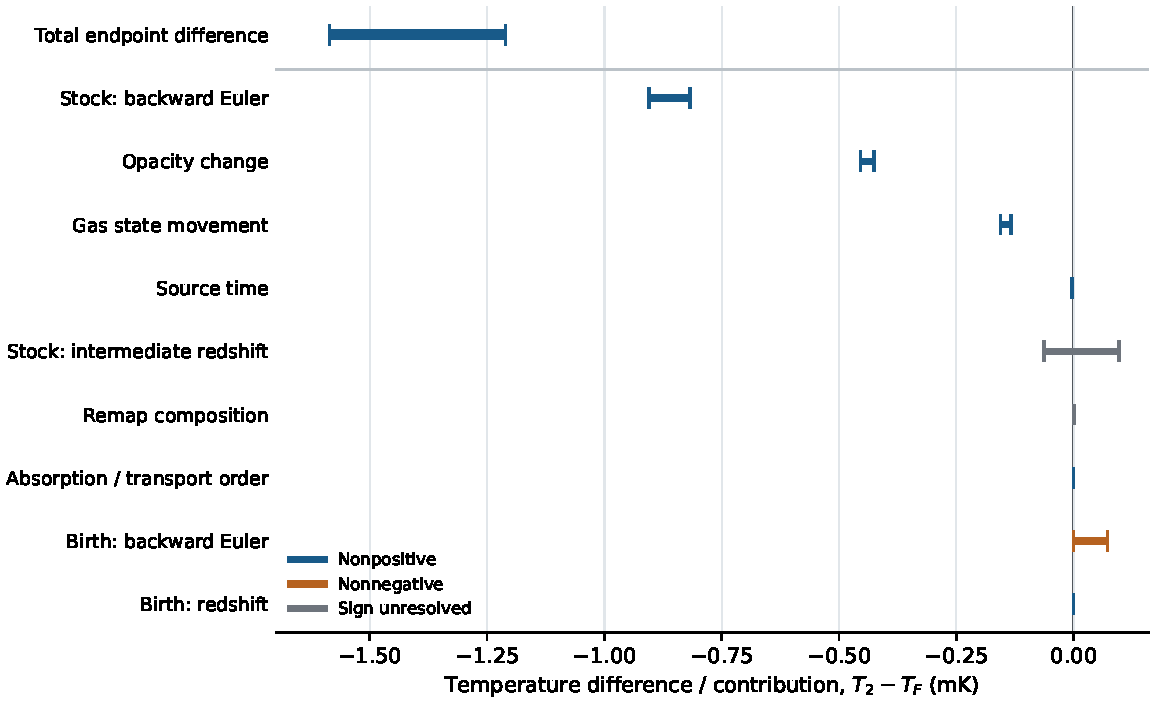
\includegraphics[width=\textwidth]{temperature_sectors.pdf}
\caption{계열 전체의 결정론적 외향 포함이며 통계적 신뢰구간이 아니다. 각 sector에 같은 inverse와 온도 분모를 적용했고 $b=0$을 포함했다. 작은 birth-redshift는 이 mK 척도에서 0에 가까우므로 정확한 부호와 값은 표 \ref{tab:birth}를 참조한다.}
\label{fig:sectors}
\end{figure}

Stock 중간 수송과 remap 합성의 포함은 0을 가로지른다. 이 계산은 그 두 항의 계열 전체 부호를 결정하지 않는다. 또한 각 행의 구간 끝점은 서로 다른 입력 선택에서 나올 수 있으므로, 행별 최악값의 합은 총 $\Delta T$의 가장 좁은 포함과 같을 필요가 없다. 총량은 동일 dependency graph에서 별도로 계산한 표 \ref{tab:gasresults}를 사용한다.

\subsection{실제 광자 endpoint와 guard 보존}
$\widehat{\Delta Z}=Z_2-A_F(g_2)Q_F$는 $g_2$에서 평가한 Full과의 차이다. 실제 Full 근의 opacity까지 옮긴 최종 차이는 각 활성 group에서
\begin{equation}
(Z_2-Z_F)_j=\widehat{\Delta Z}_j
+\frac{2ha_{2j}Q_{Fj}d_x}{D_jD_{Fj}}.
\label{eq:photonsecant}
\end{equation}
두 guard와 inactive group에는 두 번째 항이 없다. Number와 energy의 행벡터는 각각
\begin{equation}
\ell_N=(1,\ldots,1,1,0),\qquad
\ell_U=(E_0,\ldots,E_{32},0,1)
\label{eq:photonrows}
\end{equation}
이다. 33개 group과 두 guard를 모두 유지한 결과는
\begin{align}
\Delta N_\gamma&\in[-8.017117741337,-2.993772375131]\times10^{-8}
\quad[\mathrm{photons/H}],\\
\Delta U_\gamma&\in[-1.097031889614\times10^{-6},-4.091984857188\times10^{-7}]
\quad[\mathrm{eV/H}].
\label{eq:photonresults}
\end{align}
두 값은 모두 엄밀하게 음수다. 식 \eqref{eq:photonsecant}는 $d_x>0$에서 비음수의 secant 보정을 더하지만, 그 보정을 포함한 총량도 음의 구간에 남는다.\cite{app16}

Anchor ledger 역시 직접 추적했다. $\widehat{\Delta N}=\ell_N\widehat{\Delta Z}$, $\widehat{\Delta U}=\ell_U\widehat{\Delta Z}$로 두면
\begin{align}
\mathbf1^{\mathsf T}p&=-\widehat{\Delta N},\\
E^{\mathsf T}p&=(1-\rho)(E^{\mathsf T}P_1-bM_\gamma E_{24})-\widehat{\Delta U},\\
\epsilon^{\mathsf T}p&=(1-\rho)(E^{\mathsf T}P_1-bM_\gamma E_{24})
-\widehat{\Delta U}+\chi_H\widehat{\Delta N}.
\label{eq:ledgers}
\end{align}
첫 half에서 흡수된 광자가 두 번째 수송에 들어가지 않는 chronology가 중간 항을 만든다. 실제 계산의 세 ledger 잔차 포함은 모두 0을 포함한다. 이 수치 검산은 식 \eqref{eq:ledgers}의 직접 대수 유도와 함께 사용한다.

\section{실행 근거와 Wolfram/xAct 검산}\label{sec:execution}
\subsection{두 개의 bounded 산술 적용}
이번 연구는 상속된 source 값·gradient·Hessian 및 실제 root 포함에 새로운 차이식과 나머지 정리를 적용했다. 두 scientific 실행은 사전에 명령, 확인할 값, 예산을 \texttt{PRE\_RUN.json}으로 남기고, exit code·wall time·CPU·RSS·출력 hash를 기록했다. 첫 실행은 상관 잔차와 componentwise 전달, 둘째 실행은 finite endpoint 및 공통 adjoint 보정이다.

\begin{table}[H]
\centering\small
\begin{tabularx}{\textwidth}{@{}Xrrr@{}}
\toprule
적용 & Wall [s] & Peak RSS [KiB] & Exit\\\midrule
상관 residual, gas·35 photon readout & 0.465254261 & 41984 & 0\\
Endpoint Hessian, $m=2$, 공통 adjoint & 0.087223469 & 16060 & 0\\
\bottomrule
\end{tabularx}
\caption{실제 wrapper 기록. 첫 실행 user CPU는 0.402452 s다. 둘째 scientific 내부 연산 시간은 0.024816254 s이고 표는 wrapper의 측정값이다.}
\label{tab:runs}
\end{table}

원 source 및 반응 kernel 호출, 비선형 root solve, 과거 history replay는 두 실행에서 모두 0회다. Cooling cone을 통해 $k_{wHe}$를 포함한 단독 scalar 산술은 보존된 $F_w^{np}$의 포함과 부호를 사용했다. CI/RR/DR fit의 전체 재실행에 해당하지 않는다. 원 PHYS15 입력은 읽기 전용으로 유지했다. 실행과 독립 검토의 최종 상태는 이 보고서 첫 페이지의 판정 및 동봉 검토 기록에 연결한다.\cite{app16,endpoint16,sourceaudit}

\subsection{독립 심사와 채택}
독립 검토자는 후보 적용 코드를 import하지 않고 exact Fraction 산술로 18개 검산 묶음을 실행했다. 원 binary64 중심과 반경, Cramer 방식의 componentwise majorant, signed Hessian 수축, Neumann 나머지, 공통 adjoint 및 birth 부호, guard 아래의 remap을 직접 대조했다. 18개 묶음은 모두 통과했고, 일곱 심사 대상 주장에 남은 blocking finding은 없다. 최종 판정은 \texttt{PROMOTE\_SCOPED}다. 검토 실행의 wrapper wall time은 0.133782941 s, peak RSS는 27588 KiB, exit code는 0이다. 원 실행 결과의 후보 상태와 hash는 보존하고 별도 \texttt{DECISION.json}에 최종 채택을 기록했다.\cite{review16}

\subsection{실제 Wolfram 및 xAct 환경}
사용한 Wolfram은 \textbf{15.0.1 Linux x86 64-bit (2026-07-02)}다. 공식 archive \texttt{xAct\_1.3.0.tgz}를 Wolfram 세션에서 내려받고 xTensor \textbf{1.3.0}, xPerm \textbf{1.2.4}를 로드했다. 두 패키지의 표시 날짜는 2025-12-29다. 초기 MathLink canonicalization 경로의 실제 비자명한 수축은 \texttt{TranslatePerm::invalid} 등으로 완료되지 않았다. 이후 공식 문서와 개발자 지원이 안내하는 \texttt{\$xpermQ=False}를 tensor 정의 전에 설정했다. 최종 검산은 \textbf{xAct/xTensor와 xPerm의 Wolfram Language group 알고리즘}을 사용했으며 외부 canonicalizer 실행을 사용하지 않았다.\cite{xact,xactrun}

\begin{table}[H]
\centering\small
\begin{tabularx}{\textwidth}{@{}p{17mm}X r@{}}
\toprule
도구 & 확인한 항등식 & 잔차\\\midrule
xTensor & 선언한 Hessian 대칭의 canonical 처리 & 0\\
xTensor & Taylor residual 전달의 index 수축 & 0\\
xTensor & Dual residual의 목표 분자 항등식 & 0\\
xTensor & 공통 sector adjoint 항등식 & 0\\
xTensor & Hessian과 목표 covector의 수축 & 0\\
xTensor & Photon rank-one action & 0\\\midrule
Wolfram & 정확 HI 유리식 Taylor 나머지 & 0\\
Wolfram & Photon mean Jacobian과 endpoint 연결 & 0\\
Wolfram & 유한 온도 predictor 항등식 & 0\\
Wolfram & Affine 좌표변환의 vector--covector pairing & 0\\
\bottomrule
\end{tabularx}
\caption{실제 최종 실행의 여섯 tensor 및 네 scalar 결과. Tensor 결과는 \texttt{TensorAllZero=True}, \texttt{Messages=\{\}}이며 scalar 첫 네 결과는 모두 정확한 0이다.}
\label{tab:xact}
\end{table}

추가 scalar 출력 $89781/200000=0.448905$는 RR 부호의 소수 유리수 예시다. 실제 source의 binary64 literal을 대체하는 bound로 쓰지 않았다. 본문의 보조정리 \ref{lem:cooling}과 실제 적용은 각각 원 exact64 constants 및 그 외향 포함에 근거한다.

Tensor 검산의 공간은 네 gas 좌표의 affine 상태 공간이다. $C^2$에서 얻은 마지막 두 index의 대칭을 \texttt{DefTensor}에 선언한 뒤, \texttt{ToCanonical}이 그 대칭과 index 수축을 일관되게 적용하는지 확인했다. Hessian의 마지막 두 index 대칭, vector와 covector의 쌍대성 및 상수 $S$의 단위 변환을 사용하며 시공간 metric을 추가하지 않았다. xAct의 정확한 대수 결과는 미적분 가정이나 원 source interval의 유효성을 별도로 증명하지 않는다. 그 부분은 제1--8절의 정의역, 적분식과 상속된 포함으로 닫았다.

\section{문헌 대응, 확보한 범위와 다음 연결}\label{sec:literature}
\subsection{원 HH에 적용한 이론의 위치}
Exa의 다섯 검색 요청과 SciSpace의 한 문헌 질의에서 검증된 잔차 계산, goal-oriented error 및 비선형 adjoint의 1차 자료를 조사했다. 검색 결과를 정리하는 데 그치지 않고 원문 정리의 가정과 여기의 같은 COMMON 유한 endpoint 정의를 대조했다.\cite{lit16}

Rump의 verification survey는 고정 전처리, componentwise 포함 및 평균값 Jacobian을 이용하는 검증 계산의 근거를 제공한다. 이 보고서는 그 구조를 원 $C,B,q,S$에 적용하고, 원 HH의 정확 photon 유리식과 signed Hessian으로 $J-\overline A$를 구체화했다.\cite{Rump2010}

Rannacher의 dual-weighted residual 전개는 관측량에 맞춘 adjoint 가중의 이론적 배경이다. 원문은 변분 정상성, Galerkin 관계와 고차 나머지를 포함하는 경우를 다룬다. 본 연구의 유한 endpoint 증명은 그 가정을 자동으로 대입하지 않고 $\HF\in C^2$에서 식 \eqref{eq:dualresidual}과 \eqref{eq:sectoridentity}를 직접 유도했다.\cite{Rannacher2003} Alekseev--Navon의 adjoint 보정 및 truncation 나머지 전개와도 같은 문제의식을 공유하되, 여기서는 계산된 $a,L_H,q$가 실제 두 HH endpoint 사이의 오차 상한을 준다.\cite{Alekseev2005}

Endtmayer--Langer--Wick의 비선형 multigoal 논문은 부정확한 primal·dual 상태에서 잔차를 남기는 접근에 관련된다. 확인한 공개 preprint 식 (6)의 마지막 primal residual 부호는 원 정의와 직접 scalar 검산에서 불일치하는 것으로 읽혀, 그 식을 본문의 증명 전제로 사용하지 않았다. 이 좁은 관찰과 검산의 범위는 부록 \ref{app:literaturesign}에 남긴다. 최종 journal 본문에 관한 추가 주장을 하지 않는다.\cite{Endtmayer2019}

\subsection{이번 루프가 닫은 계산}
PHYS15의 상관 잔차는 실제 source jet, stage relation 및 35개 photon 성분을 통해 실행 가능한 외향 포함이 됐다. 물리적 fraction과 원 thermal map을 다시 연결하여 source 시각 bridge에 필요한 helium coefficient를 포함했고, gas와 photon endpoint 총량의 부호를 확보했다. $C^2$ 적분 나머지와 유한 Neumann 정리는 평균 inverse를 endpoint 자료로 바꿀 때의 오차를 정량화한다. 동일 adjoint의 부호를 사용한 두 birth sector는 $b>0$에서 각각 음수와 양수로 결정됐다.

모든 구간은 같은 fixed-source 계열의 포함이다. 공통 $\rho$, sparse remap coefficient, $b$, opacity 증분과 source pullback을 먼저 인수 분해했지만, 구간 곱을 거치는 전체 $\lambda,b$의 joint image를 완전히 표현한 것은 아니다. 따라서 \emph{유효한 포함}과 \emph{최적 폭}을 구별해야 한다. 현 자료는 이론 나머지의 미해결 때문이 아니라, 남은 입력 의존성에서 더 좁힐 여지가 있음을 수치적으로 드러낸다.

다음 연결은 실제로 부호가 미결정인 stock 중간 수송·remap 합성과 매개변수 응답에 집중할 수 있다. 같은 $\theta$를 공유한 implicit differentiation으로 $\partial_\theta d$를 구성하면, 이번의 sector 분해와 실제 $\lambda,b$ 민감도를 연결한다. 단순히 $\Delta T_s/b$를 매개변수 미분으로 해석하지 않고, 원 source와 incoming photon의 $\theta$ 의존성을 함께 미분해야 한다. 이번 결과가 이미 제한한 $10^{-12}$ K endpoint 나머지를 더 줄이는 반복보다 이 방향이 실제 온도 포함의 정보량을 늘리는 구체적 후속 과제다.

\subsection{다음 DAG 노드의 구성적 시작식}
다음 노드 \texttt{HH\_DEFECT\_PARAMETER\_RESPONSE}의 시작식을 이미 유도했다. $y=g_2$, $\theta\in\{\lambda,b\}$, $J_F=D_g\HF(g_F;\theta)$라 쓰면, 원 implicit 식과 상관 residual을 각각 미분하여
\begin{equation}
J_Fd_\theta=r_\theta-\int_0^1\!\left\{
D_g^2\HF(y-sd;\theta)[d,y_\theta]
+D_g\partial_\theta\HF(y-sd;\theta)d\right\}\,\dd s
\label{eq:nextresponse}
\end{equation}
를 얻는다. 이는 이미 보유한 $C^2$ jet와 1차 stage carry로 시작할 수 있다. 유한 온도 응답은
\begin{equation}
\partial_\theta\Delta T=
\frac{C_Td_{w,\theta}-T_2d_{e,\theta}-T_{2,\theta}d_e
-\Delta T\{\ell_e y_\theta-d_{e,\theta}\}}{\Pi_F}
\label{eq:nexttemperature}
\end{equation}
다. 원 source export의 \texttt{G\_g\_lambda}, \texttt{G\_g\_b} 및 PHYS09/14의 실제 1차 carry를 새 contract에 대응시켰다. 이 두 식과 입력 대응은 이번에 구성했으며, 전체 $\partial_b\Delta T$, $\partial_\lambda\Delta T$의 수치 포함은 다음 노드의 실행 과제로 남긴다.\cite{next16}

\appendix
\section{재현에 필요한 입력 대응}\label{app:inputs}
PHYS16의 원 parent는 PHYS15이며 PR50의 확인된 head는
\begin{center}\small\texttt{b4b8019c6f149035c52784aced8e9cd7f3fbb23b}\end{center}
다. 입력의 권위는 파일 안에 기록된 exact endpoints와 binary64 bits다. 저장된 outward decimal은 읽기 위한 표시로 사용한다. 표 \ref{tab:inputmap}은 줄 번호가 바뀌어도 유지되는 JSON key 또는 source symbol로 대응한다.

\begin{table}[H]
\centering\small
\begin{tabularx}{\textwidth}{@{}p{44mm}X@{}}
\toprule
원 또는 신규 자료 & 읽거나 검증한 값\\\midrule
\path{UNIFORM_ARITHMETIC.json} & 같은 $C,B,q,S$; scalar $q$ 외에 원 componentwise $B$ 사용\\
\path{SOURCE_CENTRE.json} & \texttt{A\_Gg} 중심 Full residual Jacobian\\
\path{SOURCE_BOX.json} & \texttt{G\_gg}: Full residual Hessian; \texttt{q}: HH source jet\\
\path{SOURCE_*_COMPONENTS.json} & \texttt{nonphoto}: HH·외부 photo·팽창 추가 전 gas source jet\\
\path{C2_DOMAIN.json} & convex $X$, fraction 및 온도 domain; metadata와 실제 model threshold 구별\\
\path{ft03_interval_rhs} & photo-off 호출의 CI/RR/DR 값과 모든 thermal 수정 경로\\
\path{CORRELATED_DEFECT_RESULTS.json} & 공유 factor, 두 gas·일곱 photon residual, 35성분 secant, $d$와 readout\\
\path{ENDPOINT_REMAINDER_RESULTS.json} & $J,M,L_H,a$, $m=2$, sector 및 평균 adjoint 부호 포함\\
\path{WOLFRAM_XACT_EXECUTION.json} & 실패·보완 경로와 최종 여섯 tensor·네 scalar의 원 실행 응답\\
\bottomrule
\end{tabularx}
\caption{전체 상대 경로와 각 입력·산출물의 SHA256은 동봉 manifest, intake mapping 및 각 \texttt{RUN\_RECORD.json}에 보존된다. 원 PHYS15의 기존 science suite는 재실행하지 않았다.}
\label{tab:inputmap}
\end{table}

Physical coefficient의 상세 source 대응은 \texttt{SOURCE\_COOLING\_AUDIT\_KO.md}에 남겼다. 실제 threshold bits는
$\chi_H$: \texttt{402b3266051507a6},
$\chi_I$: \texttt{4038965f20504658},
$\chi_{II}$: \texttt{404b357928e0c9da}다.
각각 표시값은 $13.598434599702$, $24.587389011$, $54.41776$ eV다. $k_B$와 $\epsilon_{eV}$도 같은 captured binary64 leaf를 사용한다. 원 $\texttt{C2\_DOMAIN}$의 짧은 threshold 배열은 반올림 metadata여서 이 상수를 다시 정의하지 않는다.

논문의 $e$는 H당 전자 수이고 $n_e=ne$는 cm$^{-3}$다. $w$, $Q$, $U_\gamma$는 각각 eV/H, photons/H, eV/H로 정규화한다. $d$와 $\HF$는 같은 gas 단위를 가진다. Hessian $H^a_{jk}$는 $[g^a]/([g^j][g^k])$ 단위이며, $S$가 등장하는 노름에서 무차원화된다. $n_T,\overline z$는 온도 \emph{분자}를 위한 covector다. 이들을 $\Pi_F$로 나누기 전 값과 온도 기여를 혼동하지 않는다.

\section{문헌의 한 부호식에 대한 제한된 검산}\label{app:literaturesign}
확인한 Endtmayer--Langer--Wick의 RICAM 공개 preprint는 $\rho(\widetilde u)=-\mathcal A(\widetilde u)$로 정의한다. 식 (6)의 마지막 primal residual 항을 $-\rho(\widetilde u)(\widetilde z)$로 읽으면 다음 scalar 예가 일치하지 않는다.\cite{Endtmayer2019,lit16}
\begin{equation}
\mathcal A(u)(v)=uv,\quad J(u)=u,\quad
u=0,\quad z=1,\quad\widetilde u=1,\quad\widetilde z=1.
\end{equation}
여기서 모든 함수는 $C^\infty$이고 dual residual과 cubic remainder가 0이다. 정확한 goal 차이는 $-1$인데 해당 표시를 적용한 우변은 $+1$이다. $L(u,z)=J(u)-\mathcal A(u)(z)$에서 직접 유도하면 마지막 항은 $+\rho(\widetilde u)(\widetilde z)$다. 실제 scalar 검산 결과와 읽은 원문 위치는 문헌 패키지에 보존했다. 이 관찰은 접근한 공개 preprint의 식과 정의에 한정하며, 접근하지 못한 최종 journal 본문의 판정으로 확대하지 않는다. 본문의 endpoint·sector 정리는 해당 식과 독립적으로 증명했다.

\begin{thebibliography}{99}\small
\bibitem{phys14} WU088\_HH 연구 기록, \emph{PHYS14: geometric isotropic source-aligned 실제 endpoint 및 공통 arithmetic 포함}. PHYS15에 보존된 \path{inputs/phys14/} 원자료, root·source·arithmetic identity와 검토 기록.

\bibitem{phys15} WU088\_HH 연구 기록, \emph{PHYS15: 동일 COMMON의 정확한 Full--two-half residual과 공통 adjoint sector}. \path{HH_PHYS15_THEORY_20261012_v1}, PHYS15 보고서·contract·handoff. 확인된 PR50 head는 부록 \ref{app:inputs}에 기록했다.

\bibitem{app16} WU088\_HH PHYS16, \emph{실제 상관 endpoint residual 적용}. \path{evidence/intake/PHYS16_APPLICATION_DERIVATION_KO.md}, \path{checks/application/run01/results/CORRELATED_DEFECT_RESULTS.json}, \texttt{PRE\_RUN} 및 \texttt{RUN\_RECORD}. 2026-10-13 KST.

\bibitem{endpoint16} WU088\_HH PHYS16, \emph{Endpoint Jacobian과 이차 remainder에 의한 관측량 포함}. \path{theory/ENDPOINT_REMAINDER_THEORY_KO.md}; \path{checks/endpoint/ENDPOINT_HESSIAN_READOUT.json}; \path{checks/endpoint/application01/ENDPOINT_REMAINDER_RESULTS.json}. 2026-10-13 KST.

\bibitem{sourceaudit} WU088\_HH PHYS16, \emph{원 source cooling-cone 교차점검}. \path{evidence/intake/SOURCE_COOLING_AUDIT_KO.md}. 원 FT03 CI/RR/DR thermal symbol·상수·domain·export 순서와 source hash를 포함한 읽기 감사. 2026-10-13 KST.

\bibitem{review16} WU088\_HH PHYS16, \emph{독립 이론·산술 심사와 최종 채택}. \path{review/INDEPENDENT_REVIEW.json}, \path{review/INDEPENDENT_ARITHMETIC_RESULTS.json}, \path{review/independent_arithmetic_review.py}, \path{review/DECISION.json}. 18개 검산 묶음 통과, \texttt{PROMOTE\_SCOPED}, 2026-10-13 KST.

\bibitem{next16} WU088\_HH PHYS16, \emph{다음 매개변수 응답의 시작식과 입력 계약}. \path{theory/NEXT_PARAMETER_RESPONSE_PROPOSAL_KO.md}, \path{contracts/PARAMETER_RESPONSE_CONTRACT.json}, \path{NEXT_DAG.json}. 2026-10-13 KST.

\bibitem{Rump2010} S. M. Rump, ``Verification methods: Rigorous results using floating-point arithmetic,'' \emph{Acta Numerica} \textbf{19} (2010), 287--449. DOI: \href{https://doi.org/10.1017/S096249291000005X}{10.1017/S096249291000005X}. \href{https://www.tuhh.de/ti3/paper/rump/Ru10.pdf}{저자 공개 원문}; Theorems 10.2, 10.6, 10.8 및 Sections 11.3--11.6, 13.

\bibitem{Rannacher2003} R. Rannacher, ``Adaptive Finite Element Methods for Partial Differential Equations,'' arXiv:math/0305006 (2003), ICM 2002 lecture. \url{https://arxiv.org/pdf/math/0305006}. Propositions 1--2 및 residual--adjoint 전개.

\bibitem{Endtmayer2019} B. Endtmayer, U. Langer, T. Wick, ``Multigoal-oriented error estimates for non-linear problems,'' \emph{Journal of Numerical Mathematics} \textbf{27}(4) (2019), 215--236. DOI: \href{https://doi.org/10.1515/jnma-2018-0038}{10.1515/jnma-2018-0038}. 실제 확인 원문: \href{https://www.ricam.oeaw.ac.at/files/reports/18/rep18-08.pdf}{RICAM Report 2018-08}, Theorem 3.1과 Remarks 3.2--3.4. 부록 \ref{app:literaturesign}의 범위를 따른다.

\bibitem{Alekseev2005} A. K. Alekseev, I. M. Navon, ``Adjoint correction and bounding of error using Lagrange form of truncation term,'' \emph{Computers \& Mathematics with Applications} \textbf{50} (2005), 1311--1332. DOI: \href{https://doi.org/10.1016/j.camwa.2005.05.004}{10.1016/j.camwa.2005.05.004}. \href{https://people.sc.fsu.edu/~inavon/pubs/CAM2005.pdf}{저자 공개 원문}, Section 2.1.

\bibitem{xact} J. M. Martín-García 외, \emph{xAct / xTensor 공식 자료}. \url{https://xact.es/}; \url{https://xact.es/download.html}; \href{https://xact.es/Documentation/HTML/HTMLLinks/xTensor/ToCanonical.nb.html}{ToCanonical 문서}; \href{https://groups.google.com/g/xact/c/U6vGTjEZVDE}{xAct 개발자 지원의 내부 group backend 안내}. 2026-10-13 KST 확인.

\bibitem{xactrun} WU088\_HH PHYS16, \emph{Wolfram/xAct 실제 실행 기록}. \path{checks/wolfram/WOLFRAM_XACT_EXECUTION.json}, \path{checks/wolfram/endpoint_tensor_checks.wl}. 공식 archive SHA256:
\texttt{7a6c5f600868a3922668b020a15c0692f}\\
\texttt{76574ff2a559808c62d460cef1b07be}.

\bibitem{lit16} WU088\_HH PHYS16, \emph{문헌 조사와 endpoint bridge}. \path{literature/LITERATURE_REVIEW_KO.md}, \path{literature/ENDPOINT_BRIDGE_NOTE_KO.md}, 검색 provenance·manifest 및 \path{literature/PREPRINT_SIGN_CHECK.json}. Exa·SciSpace 검색과 1차 원문 검토, 2026-10-13 KST.
\end{thebibliography}

\end{document}
